\section{C}
\subsection*{Material ID: mp-cejdg}
\textbf{Constante Dieléctrica ($\epsilon_{total}$):} 6.60 \\[0.5em]
\begin{table}[h!]
\centering
\begin{tabular}{lcc}
\toprule
\textbf{Métrica} & \textbf{Lámina (Plate)} & \textbf{Cilindros (Rod)} \\
\midrule
Bandgaps ($a/\lambda$) & Ninguno & Ninguno \\
Resonancias & 36 & 36 \\
\bottomrule
\end{tabular}
\end{table}
\begin{figure}[H]
\centering
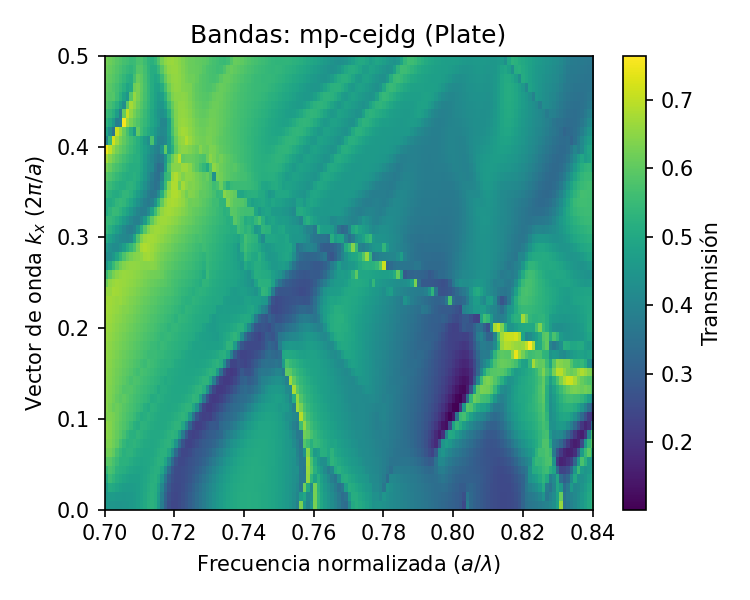
\includegraphics[width=0.48\textwidth]{figures/mp-cejdg_plate.png}
\hfill
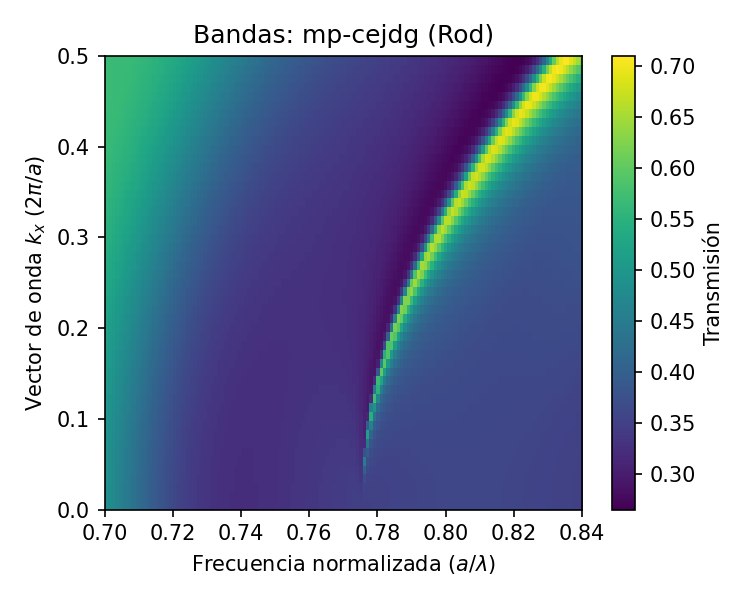
\includegraphics[width=0.48\textwidth]{figures/mp-cejdg_rod.png}
\caption{Estructuras de bandas fotónicas para mp-cejdg. Izquierda: Lámina. Derecha: Cilindros.}
\end{figure}
\vspace{1em}
\hrule
\vspace{1em}
\subsection*{Material ID: mp-co}
\textbf{Constante Dieléctrica ($\epsilon_{total}$):} 5.83 \\[0.5em]
\begin{table}[h!]
\centering
\begin{tabular}{lcc}
\toprule
\textbf{Métrica} & \textbf{Lámina (Plate)} & \textbf{Cilindros (Rod)} \\
\midrule
Bandgaps ($a/\lambda$) & Ninguno & Ninguno \\
Resonancias & 36 & 36 \\
\bottomrule
\end{tabular}
\end{table}
\begin{figure}[H]
\centering
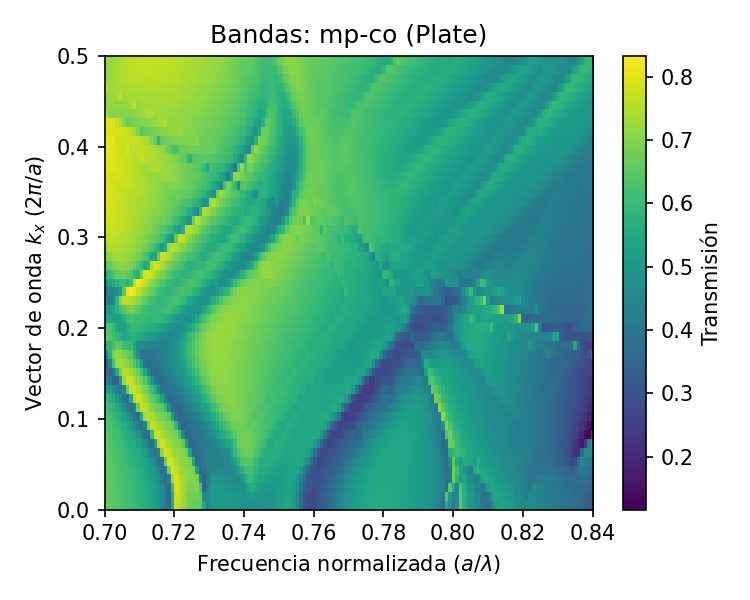
\includegraphics[width=0.48\textwidth]{figures/mp-co_plate.png}
\hfill
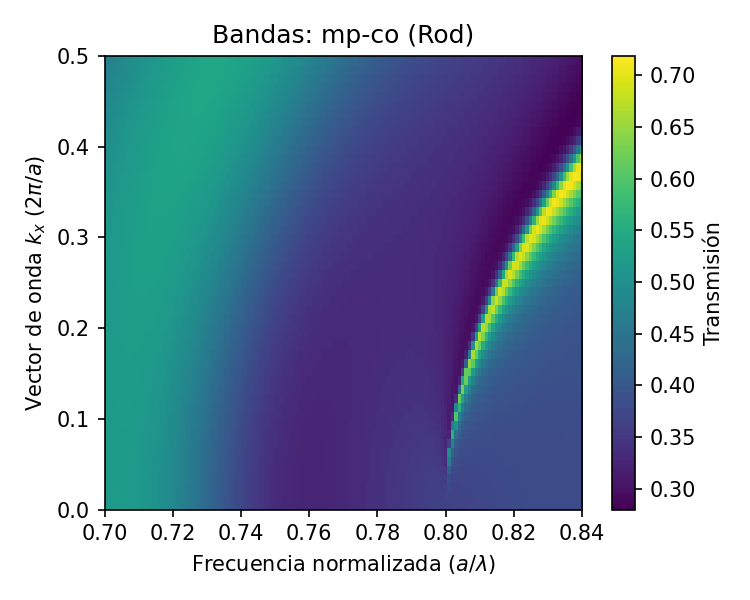
\includegraphics[width=0.48\textwidth]{figures/mp-co_rod.png}
\caption{Estructuras de bandas fotónicas para mp-co. Izquierda: Lámina. Derecha: Cilindros.}
\end{figure}
\vspace{1em}
\hrule
\vspace{1em}
\clearpage